%qqqqqqqqqqqqqqqqqqqqqqqqqqqqqqqqqqqqqqqqqqqqqqqqqqqqqqqqqqqqqqqqqqqqqqqqq
%Quote
\begin{savequote}[50mm]
%‘‘El cosmos es todo lo que es, todo lo que fue y todo lo que será. Nuestras 
%más ligeras contemplaciones del cosmos nos hacen estremecer: Sentimos como 
%un cosquilleo nos llena los nervios, una voz muda, una ligera sensación como
%de un recuerdo lejano o como si cayéramos desde gran altura. Sabemos que nos
%aproximamos al más grande de los misterios.’’
%\qauthor{Carl Sagan}
\end{savequote}
%qqqqqqqqqqqqqqqqqqqqqqqqqqqqqqqqqqqqqqqqqqqqqqqqqqqqqqqqqqqqqqqqqqqqqqqqq




%#########################################################################
\chapter{Alineamiento de AGNs con su entorno a gran escala}
\label{cha:cosmic_web}

En esta sección se presentan los resultados obtenidos en la búsqueda de posible alineamiento del espín de los AGNs y el entorno cosmológico al cual pertenecen. Con al fin de poder llevar a cabo este propósito, se hace uso de: dos simulaciones cosmológicas ({\it{Cosmo01}} y {\it{Cosmo02}}), los los autovalores, autovectores, sobre densidades obtenidos con el método de T-Web y el catálogo FoF. A continuación se presentan las características de la simulaciones y de los resultados obtenidos.

%------------------------------------------------
\section{Características de las simulaciones}
\label{sec: propiedades en las simulaciones}
%------------------------------------------------

En la simulación hay parámetros o valores que dan información de la dinámica del sistema,  que arrojan criterios suficientes para decidir si lo obtenido está en acuerdo con los modelos físicos propuestos. 
Conforme a esto, se pretende realizar un análisis a la distribución de masa (función de masa) de los halos de materia, BHs y de estrellas. 

%------------------------------------------------
\subsection{ Función de masa}
\label{subsec: funcion de masa}
%------------------------------------------------
La función de masa es uno de los parámetros de control más contundentes en el análisis de las simulaciones. Bajo la teoría de formación y evolución de galaxias se tiene que los objetos con baja masa son más abundantes. En los procesos evolutivos de las galaxias la interacción es jerárquica con respecto a la masa, las galaxias más masivas tiene una mayor probabilidad en fusionarse con otras debido a su gran potencial gravitacional. Con base a esto las funciones de masa de las galaxias debe decrecer a medida que se aumentan las masas. 

\begin{figure}
 \centering
  \subfloat{
   \label{fig: función de masa BHs}
    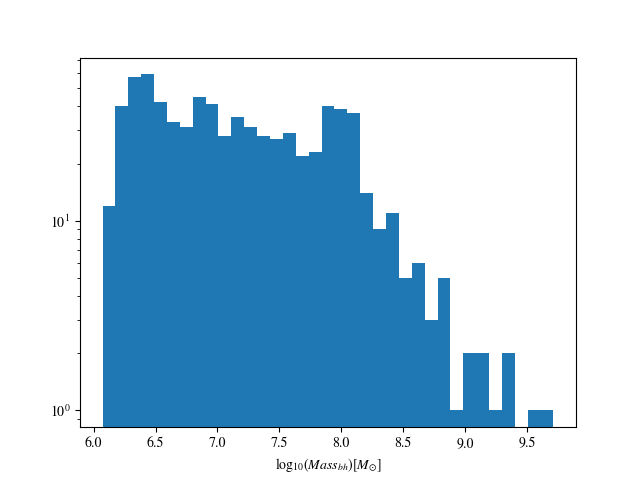
\includegraphics[width=0.31\textwidth]{./figures/6_Resultados/cosmo01/histo_Mass_bh.png}}
  \subfloat{
   \label{fig: función de masa halos}
    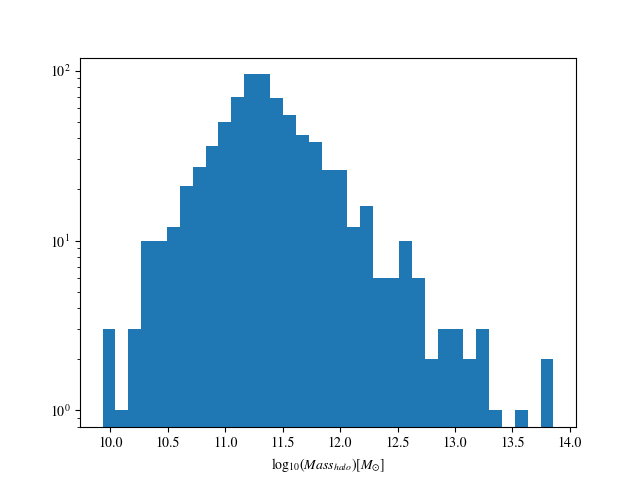
\includegraphics[width=0.31\textwidth]{./figures/6_Resultados/cosmo01/histo_Mass_halos.png}}
  \subfloat{
   \label{fig: función de masa estelar}
    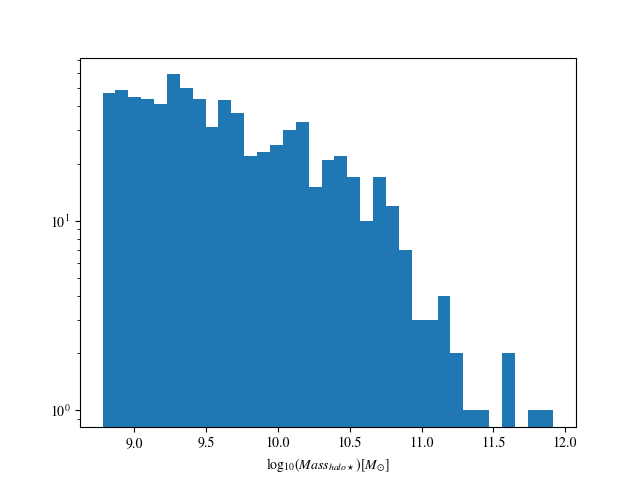
\includegraphics[width=0.31\textwidth]{./figures/6_Resultados/cosmo01/histo_Mass_stelar.png}}
 \caption{Funciones de masa para agujeros negros, halos y masa estelar, estas información da cuenta del número de objetos con una masa determinada, esto se realizo para {\it{Cosmo01}}. }
 \label{fig: Funciones de masa}
\end{figure}
 HACER LO MISMO PARA COSMO 2

Al observar las figuras (\ref{fig: Funciones de masa}, ... ), es posible concluir que los resultados de la simulación con congruentes con la teoría y con las observaciones. 








%***********************************************************************